\documentclass[twoside]{book}

% Packages required by doxygen
\usepackage{fixltx2e}
\usepackage{calc}
\usepackage{doxygen}
\usepackage[export]{adjustbox} % also loads graphicx
\usepackage{graphicx}
\usepackage[utf8]{inputenc}
\usepackage{makeidx}
\usepackage{multicol}
\usepackage{multirow}
\PassOptionsToPackage{warn}{textcomp}
\usepackage{textcomp}
\usepackage[nointegrals]{wasysym}
\usepackage[table]{xcolor}

% Font selection
\usepackage[T1]{fontenc}
\usepackage[scaled=.90]{helvet}
\usepackage{courier}
\usepackage{amssymb}
\usepackage{sectsty}
\renewcommand{\familydefault}{\sfdefault}
\allsectionsfont{%
  \fontseries{bc}\selectfont%
  \color{darkgray}%
}
\renewcommand{\DoxyLabelFont}{%
  \fontseries{bc}\selectfont%
  \color{darkgray}%
}
\newcommand{\+}{\discretionary{\mbox{\scriptsize$\hookleftarrow$}}{}{}}

% Page & text layout
\usepackage{geometry}
\geometry{%
  a4paper,%
  top=2.5cm,%
  bottom=2.5cm,%
  left=2.5cm,%
  right=2.5cm%
}
\tolerance=750
\hfuzz=15pt
\hbadness=750
\setlength{\emergencystretch}{15pt}
\setlength{\parindent}{0cm}
\setlength{\parskip}{3ex plus 2ex minus 2ex}
\makeatletter
\renewcommand{\paragraph}{%
  \@startsection{paragraph}{4}{0ex}{-1.0ex}{1.0ex}{%
    \normalfont\normalsize\bfseries\SS@parafont%
  }%
}
\renewcommand{\subparagraph}{%
  \@startsection{subparagraph}{5}{0ex}{-1.0ex}{1.0ex}{%
    \normalfont\normalsize\bfseries\SS@subparafont%
  }%
}
\makeatother

% Headers & footers
\usepackage{fancyhdr}
\pagestyle{fancyplain}
\fancyhead[LE]{\fancyplain{}{\bfseries\thepage}}
\fancyhead[CE]{\fancyplain{}{}}
\fancyhead[RE]{\fancyplain{}{\bfseries\leftmark}}
\fancyhead[LO]{\fancyplain{}{\bfseries\rightmark}}
\fancyhead[CO]{\fancyplain{}{}}
\fancyhead[RO]{\fancyplain{}{\bfseries\thepage}}
\fancyfoot[LE]{\fancyplain{}{}}
\fancyfoot[CE]{\fancyplain{}{}}
\fancyfoot[RE]{\fancyplain{}{\bfseries\scriptsize Generated by Doxygen }}
\fancyfoot[LO]{\fancyplain{}{\bfseries\scriptsize Generated by Doxygen }}
\fancyfoot[CO]{\fancyplain{}{}}
\fancyfoot[RO]{\fancyplain{}{}}
\renewcommand{\footrulewidth}{0.4pt}
\renewcommand{\chaptermark}[1]{%
  \markboth{#1}{}%
}
\renewcommand{\sectionmark}[1]{%
  \markright{\thesection\ #1}%
}

% Indices & bibliography
\usepackage{natbib}
\usepackage[titles]{tocloft}
\setcounter{tocdepth}{3}
\setcounter{secnumdepth}{5}
\makeindex

% Hyperlinks (required, but should be loaded last)
\usepackage{ifpdf}
\ifpdf
  \usepackage[pdftex,pagebackref=true]{hyperref}
\else
  \usepackage[ps2pdf,pagebackref=true]{hyperref}
\fi
\hypersetup{%
  colorlinks=true,%
  linkcolor=blue,%
  citecolor=blue,%
  unicode%
}

% Custom commands
\newcommand{\clearemptydoublepage}{%
  \newpage{\pagestyle{empty}\cleardoublepage}%
}

\usepackage{caption}
\captionsetup{labelsep=space,justification=centering,font={bf},singlelinecheck=off,skip=4pt,position=top}

%===== C O N T E N T S =====

\begin{document}

% Titlepage & ToC
\hypersetup{pageanchor=false,
             bookmarksnumbered=true,
             pdfencoding=unicode
            }
\pagenumbering{roman}
\begin{titlepage}
\vspace*{7cm}
\begin{center}%
{\Large hoppin }\\
\vspace*{1cm}
{\large Generated by Doxygen 1.8.11}\\
\end{center}
\end{titlepage}
\clearemptydoublepage
\tableofcontents
\clearemptydoublepage
\pagenumbering{arabic}
\hypersetup{pageanchor=true}

%--- Begin generated contents ---
\chapter{Namespace Index}
\section{Packages}
Here are the packages with brief descriptions (if available)\+:\begin{DoxyCompactList}
\item\contentsline{section}{\hyperlink{namespacehoppin}{hoppin} }{\pageref{namespacehoppin}}{}
\item\contentsline{section}{\hyperlink{namespacehoppin_1_1_game_information}{hoppin.\+Game\+Information} }{\pageref{namespacehoppin_1_1_game_information}}{}
\end{DoxyCompactList}

\chapter{Hierarchical Index}
\section{Class Hierarchy}
This inheritance list is sorted roughly, but not completely, alphabetically\+:\begin{DoxyCompactList}
\item \contentsline{section}{hoppin.\+Abstract\+Player}{\pageref{classhoppin_1_1_abstract_player}}{}
\item Form\begin{DoxyCompactList}
\item \contentsline{section}{hoppin.\+Hoppin\+UI}{\pageref{classhoppin_1_1_hoppin_u_i}}{}
\end{DoxyCompactList}
\item \contentsline{section}{hoppin.\+Game\+System.\+Game\+Manager}{\pageref{classhoppin_1_1_game_system_1_1_game_manager}}{}
\item \contentsline{section}{hoppin.\+Game\+System.\+Game\+State}{\pageref{classhoppin_1_1_game_system_1_1_game_state}}{}
\begin{DoxyCompactList}
\item \contentsline{section}{hoppin.\+Game\+System.\+Game\+Manager.\+New\+Game\+State}{\pageref{classhoppin_1_1_game_system_1_1_game_manager_1_1_new_game_state}}{}
\end{DoxyCompactList}
\item \contentsline{section}{hoppin.\+Game\+System.\+Judgement}{\pageref{classhoppin_1_1_game_system_1_1_judgement}}{}
\item \contentsline{section}{hoppin.\+Game\+System.\+Player\+Data}{\pageref{classhoppin_1_1_game_system_1_1_player_data}}{}
\item \contentsline{section}{hoppin.\+Game\+System.\+Position}{\pageref{classhoppin_1_1_game_system_1_1_position}}{}
\end{DoxyCompactList}

\chapter{Class Index}
\section{Class List}
Here are the classes, structs, unions and interfaces with brief descriptions\+:\begin{DoxyCompactList}
\item\contentsline{section}{\hyperlink{classhoppin_1_1_abstract_player}{hoppin.\+Abstract\+Player} }{\pageref{classhoppin_1_1_abstract_player}}{}
\item\contentsline{section}{\hyperlink{classhoppin_1_1_game_system_1_1_game_manager}{hoppin.\+Game\+System.\+Game\+Manager} }{\pageref{classhoppin_1_1_game_system_1_1_game_manager}}{}
\item\contentsline{section}{\hyperlink{classhoppin_1_1_game_system_1_1_game_state}{hoppin.\+Game\+System.\+Game\+State} }{\pageref{classhoppin_1_1_game_system_1_1_game_state}}{}
\item\contentsline{section}{\hyperlink{classhoppin_1_1_hoppin_u_i}{hoppin.\+Hoppin\+UI} }{\pageref{classhoppin_1_1_hoppin_u_i}}{}
\item\contentsline{section}{\hyperlink{classhoppin_1_1_game_system_1_1_judgement}{hoppin.\+Game\+System.\+Judgement} }{\pageref{classhoppin_1_1_game_system_1_1_judgement}}{}
\item\contentsline{section}{\hyperlink{classhoppin_1_1_game_system_1_1_game_manager_1_1_new_game_state}{hoppin.\+Game\+System.\+Game\+Manager.\+New\+Game\+State} }{\pageref{classhoppin_1_1_game_system_1_1_game_manager_1_1_new_game_state}}{}
\item\contentsline{section}{\hyperlink{classhoppin_1_1_game_system_1_1_player_data}{hoppin.\+Game\+System.\+Player\+Data} }{\pageref{classhoppin_1_1_game_system_1_1_player_data}}{}
\item\contentsline{section}{\hyperlink{classhoppin_1_1_game_system_1_1_position}{hoppin.\+Game\+System.\+Position} }{\pageref{classhoppin_1_1_game_system_1_1_position}}{}
\end{DoxyCompactList}

\chapter{Namespace Documentation}
\hypertarget{namespacehoppin}{}\section{hoppin 名前空間}
\label{namespacehoppin}\index{hoppin@{hoppin}}
\subsection*{名前空間}
\begin{DoxyCompactItemize}
\item 
namespace \hyperlink{namespacehoppin_1_1_properties}{Properties}
\end{DoxyCompactItemize}
\subsection*{クラス}
\begin{DoxyCompactItemize}
\item 
class \hyperlink{classhoppin_1_1_abstract_player}{Abstract\+Player}
\item 
class \hyperlink{classhoppin_1_1_hoppin_u_i}{Hoppin\+UI}
\item 
class {\bfseries Program}
\begin{DoxyCompactList}\small\item\em ゲームシステムのクラス \end{DoxyCompactList}\item 
class \hyperlink{classhoppin_1_1_sample_player}{Sample\+Player}
\end{DoxyCompactItemize}

\hypertarget{namespacehoppin_1_1_game_system}{}\section{hoppin.\+Game\+System 名前空間}
\label{namespacehoppin_1_1_game_system}\index{hoppin.\+Game\+System@{hoppin.\+Game\+System}}
\subsection*{クラス}
\begin{DoxyCompactItemize}
\item 
class \hyperlink{classhoppin_1_1_game_system_1_1_game_state}{Game\+State}
\item 
class \hyperlink{classhoppin_1_1_game_system_1_1_judgement}{Judgement}
\end{DoxyCompactItemize}
\subsection*{列挙型}
\begin{DoxyCompactItemize}
\item 
enum \hyperlink{namespacehoppin_1_1_game_system_a09ca9399921bb6094069df368b7c3f0f}{Player\+Move} \+: int \{ \hyperlink{namespacehoppin_1_1_game_system_a09ca9399921bb6094069df368b7c3f0fa46c48bec0d282018b9d167eef7711b2c}{Player\+Move.\+up}, 
\hyperlink{namespacehoppin_1_1_game_system_a09ca9399921bb6094069df368b7c3f0fa74e8333ad11685ff3bdae589c8f6e34d}{Player\+Move.\+down}, 
\hyperlink{namespacehoppin_1_1_game_system_a09ca9399921bb6094069df368b7c3f0fa811882fecd5c7618d7099ebbd39ea254}{Player\+Move.\+left}, 
\hyperlink{namespacehoppin_1_1_game_system_a09ca9399921bb6094069df368b7c3f0fa7c4f29407893c334a6cb7a87bf045c0d}{Player\+Move.\+right}
 \}
\end{DoxyCompactItemize}


\subsection{列挙型詳解}
\index{hoppin\+::\+Game\+System@{hoppin\+::\+Game\+System}!Player\+Move@{Player\+Move}}
\index{Player\+Move@{Player\+Move}!hoppin\+::\+Game\+System@{hoppin\+::\+Game\+System}}
\subsubsection[{\texorpdfstring{Player\+Move}{PlayerMove}}]{\setlength{\rightskip}{0pt plus 5cm}enum {\bf hoppin.\+Game\+System.\+Player\+Move} \+: int\hspace{0.3cm}{\ttfamily [strong]}}\hypertarget{namespacehoppin_1_1_game_system_a09ca9399921bb6094069df368b7c3f0f}{}\label{namespacehoppin_1_1_game_system_a09ca9399921bb6094069df368b7c3f0f}
\begin{Desc}
\item[列挙値]\par
\begin{description}
\index{up@{up}!hoppin\+::\+Game\+System@{hoppin\+::\+Game\+System}}\index{hoppin\+::\+Game\+System@{hoppin\+::\+Game\+System}!up@{up}}\item[{\em 
up\hypertarget{namespacehoppin_1_1_game_system_a09ca9399921bb6094069df368b7c3f0fa46c48bec0d282018b9d167eef7711b2c}{}\label{namespacehoppin_1_1_game_system_a09ca9399921bb6094069df368b7c3f0fa46c48bec0d282018b9d167eef7711b2c}
}]\index{down@{down}!hoppin\+::\+Game\+System@{hoppin\+::\+Game\+System}}\index{hoppin\+::\+Game\+System@{hoppin\+::\+Game\+System}!down@{down}}\item[{\em 
down\hypertarget{namespacehoppin_1_1_game_system_a09ca9399921bb6094069df368b7c3f0fa74e8333ad11685ff3bdae589c8f6e34d}{}\label{namespacehoppin_1_1_game_system_a09ca9399921bb6094069df368b7c3f0fa74e8333ad11685ff3bdae589c8f6e34d}
}]\index{left@{left}!hoppin\+::\+Game\+System@{hoppin\+::\+Game\+System}}\index{hoppin\+::\+Game\+System@{hoppin\+::\+Game\+System}!left@{left}}\item[{\em 
left\hypertarget{namespacehoppin_1_1_game_system_a09ca9399921bb6094069df368b7c3f0fa811882fecd5c7618d7099ebbd39ea254}{}\label{namespacehoppin_1_1_game_system_a09ca9399921bb6094069df368b7c3f0fa811882fecd5c7618d7099ebbd39ea254}
}]\index{right@{right}!hoppin\+::\+Game\+System@{hoppin\+::\+Game\+System}}\index{hoppin\+::\+Game\+System@{hoppin\+::\+Game\+System}!right@{right}}\item[{\em 
right\hypertarget{namespacehoppin_1_1_game_system_a09ca9399921bb6094069df368b7c3f0fa7c4f29407893c334a6cb7a87bf045c0d}{}\label{namespacehoppin_1_1_game_system_a09ca9399921bb6094069df368b7c3f0fa7c4f29407893c334a6cb7a87bf045c0d}
}]\end{description}
\end{Desc}


 Game\+State.\+cs の 9 行目に定義があります。


\hypertarget{namespacehoppin_1_1_game_system_1_1_u_i}{}\section{hoppin.\+Game\+System.\+UI Namespace Reference}
\label{namespacehoppin_1_1_game_system_1_1_u_i}\index{hoppin.\+Game\+System.\+UI@{hoppin.\+Game\+System.\+UI}}
\subsection*{Classes}
\begin{DoxyCompactItemize}
\item 
class \hyperlink{classhoppin_1_1_game_system_1_1_u_i_1_1_background}{Background}
\item 
class \hyperlink{classhoppin_1_1_game_system_1_1_u_i_1_1_battle_field}{Battle\+Field}
\item 
class \hyperlink{classhoppin_1_1_game_system_1_1_u_i_1_1_field_block}{Field\+Block}
\item 
class \hyperlink{classhoppin_1_1_game_system_1_1_u_i_1_1_field_panel}{Field\+Panel}
\item 
class \hyperlink{classhoppin_1_1_game_system_1_1_u_i_1_1_score_board}{Score\+Board}
\item 
class \hyperlink{classhoppin_1_1_game_system_1_1_u_i_1_1_score_panel}{Score\+Panel}
\item 
class \hyperlink{classhoppin_1_1_game_system_1_1_u_i_1_1_style}{Style}
\item 
class \hyperlink{classhoppin_1_1_game_system_1_1_u_i_1_1_turn_board}{Turn\+Board}
\end{DoxyCompactItemize}

\hypertarget{namespacehoppin_1_1_properties}{}\section{hoppin.\+Properties Namespace Reference}
\label{namespacehoppin_1_1_properties}\index{hoppin.\+Properties@{hoppin.\+Properties}}
\subsection*{Classes}
\begin{DoxyCompactItemize}
\item 
class {\bfseries Resources}
\begin{DoxyCompactList}\small\item\em ローカライズされた文字列などを検索するための、厳密に型指定されたリソース クラスです。 \end{DoxyCompactList}\item 
class {\bfseries Settings}
\end{DoxyCompactItemize}

\chapter{Class Documentation}
\hypertarget{classhoppin_1_1_abstract_player}{}\section{hoppin.\+Abstract\+Player クラス}
\label{classhoppin_1_1_abstract_player}\index{hoppin.\+Abstract\+Player@{hoppin.\+Abstract\+Player}}
hoppin.\+Abstract\+Player の継承関係図\begin{figure}[H]
\begin{center}
\leavevmode
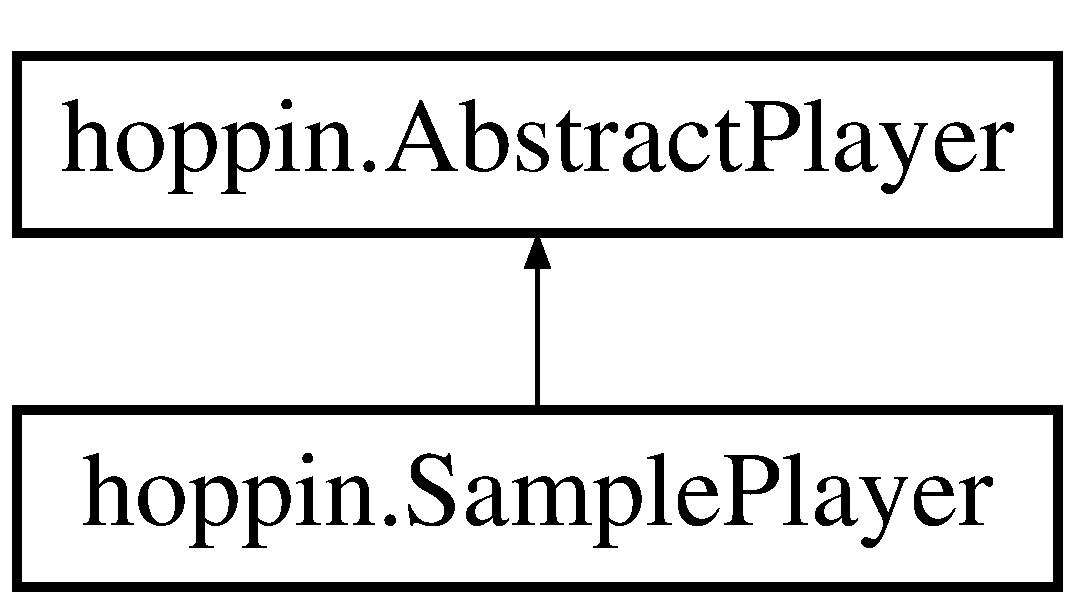
\includegraphics[height=2.000000cm]{da/d2e/classhoppin_1_1_abstract_player}
\end{center}
\end{figure}
\subsection*{公開メンバ関数}
\begin{DoxyCompactItemize}
\item 
abstract Player\+Move \hyperlink{classhoppin_1_1_abstract_player_a0f8f66f25014638ed78e82b294b4b306}{move} ()
\end{DoxyCompactItemize}


\subsection{詳解}


 Abstract\+Player.\+cs の 9 行目に定義があります。



\subsection{メソッド詳解}
\index{hoppin\+::\+Abstract\+Player@{hoppin\+::\+Abstract\+Player}!move@{move}}
\index{move@{move}!hoppin\+::\+Abstract\+Player@{hoppin\+::\+Abstract\+Player}}
\subsubsection[{\texorpdfstring{move()}{move()}}]{\setlength{\rightskip}{0pt plus 5cm}abstract Player\+Move hoppin.\+Abstract\+Player.\+move (
\begin{DoxyParamCaption}
{}
\end{DoxyParamCaption}
)\hspace{0.3cm}{\ttfamily [pure virtual]}}\hypertarget{classhoppin_1_1_abstract_player_a0f8f66f25014638ed78e82b294b4b306}{}\label{classhoppin_1_1_abstract_player_a0f8f66f25014638ed78e82b294b4b306}


このクラス詳解は次のファイルから抽出されました\+:\begin{DoxyCompactItemize}
\item 
Game\+System/\hyperlink{_abstract_player_8cs}{Abstract\+Player.\+cs}\end{DoxyCompactItemize}

\hypertarget{classhoppin_1_1_game_system_1_1_u_i_1_1_background}{}\section{hoppin.\+Game\+System.\+U\+I.\+Background Class Reference}
\label{classhoppin_1_1_game_system_1_1_u_i_1_1_background}\index{hoppin.\+Game\+System.\+U\+I.\+Background@{hoppin.\+Game\+System.\+U\+I.\+Background}}
\subsection*{Public Member Functions}
\begin{DoxyCompactItemize}
\item 
void {\bfseries draw} (Paint\+Event\+Args e)\hypertarget{classhoppin_1_1_game_system_1_1_u_i_1_1_background_ac3184f74ee57490c21ea6a3dab447608}{}\label{classhoppin_1_1_game_system_1_1_u_i_1_1_background_ac3184f74ee57490c21ea6a3dab447608}

\end{DoxyCompactItemize}


The documentation for this class was generated from the following file\+:\begin{DoxyCompactItemize}
\item 
Game\+System/\+U\+I/Background.\+cs\end{DoxyCompactItemize}

\hypertarget{classhoppin_1_1_game_system_1_1_u_i_1_1_battle_field}{}\section{hoppin.\+Game\+System.\+U\+I.\+Battle\+Field Class Reference}
\label{classhoppin_1_1_game_system_1_1_u_i_1_1_battle_field}\index{hoppin.\+Game\+System.\+U\+I.\+Battle\+Field@{hoppin.\+Game\+System.\+U\+I.\+Battle\+Field}}
\subsection*{Public Member Functions}
\begin{DoxyCompactItemize}
\item 
{\bfseries Battle\+Field} (\hyperlink{classhoppin_1_1_game_system_1_1_game_state}{Game\+State} game\+State)\hypertarget{classhoppin_1_1_game_system_1_1_u_i_1_1_battle_field_ad004f0d20da5a52cdbae4e0a775e9136}{}\label{classhoppin_1_1_game_system_1_1_u_i_1_1_battle_field_ad004f0d20da5a52cdbae4e0a775e9136}

\item 
void {\bfseries draw\+Blank\+Field} (Paint\+Event\+Args e)\hypertarget{classhoppin_1_1_game_system_1_1_u_i_1_1_battle_field_a3e68abe57917a30fa2710d58ece951c8}{}\label{classhoppin_1_1_game_system_1_1_u_i_1_1_battle_field_a3e68abe57917a30fa2710d58ece951c8}

\end{DoxyCompactItemize}


The documentation for this class was generated from the following file\+:\begin{DoxyCompactItemize}
\item 
Game\+System/\+U\+I/Battle\+Field.\+cs\end{DoxyCompactItemize}

\hypertarget{classhoppin_1_1_game_system_1_1_u_i_1_1_field_block}{}\section{hoppin.\+Game\+System.\+U\+I.\+Field\+Block Class Reference}
\label{classhoppin_1_1_game_system_1_1_u_i_1_1_field_block}\index{hoppin.\+Game\+System.\+U\+I.\+Field\+Block@{hoppin.\+Game\+System.\+U\+I.\+Field\+Block}}
\subsection*{Public Member Functions}
\begin{DoxyCompactItemize}
\item 
void {\bfseries draw} (Paint\+Event\+Args e, int x, int y, Block\+Type block\+Type)\hypertarget{classhoppin_1_1_game_system_1_1_u_i_1_1_field_block_a8b1e67b9c2bc0b569ec2894dcd420a37}{}\label{classhoppin_1_1_game_system_1_1_u_i_1_1_field_block_a8b1e67b9c2bc0b569ec2894dcd420a37}

\end{DoxyCompactItemize}


The documentation for this class was generated from the following file\+:\begin{DoxyCompactItemize}
\item 
hoppin/\+Game\+System/\+U\+I/Field\+Block.\+cs\end{DoxyCompactItemize}

\hypertarget{classhoppin_1_1_game_system_1_1_game_manager}{}\section{hoppin.\+Game\+System.\+Game\+Manager Class Reference}
\label{classhoppin_1_1_game_system_1_1_game_manager}\index{hoppin.\+Game\+System.\+Game\+Manager@{hoppin.\+Game\+System.\+Game\+Manager}}
\subsection*{Public Member Functions}
\begin{DoxyCompactItemize}
\item 
void \hyperlink{classhoppin_1_1_game_system_1_1_game_manager_a3b7f650329b12f373ef3d4077bf6d3a3}{Process\+Game} ()
\end{DoxyCompactItemize}


\subsection{Member Function Documentation}
\index{hoppin\+::\+Game\+System\+::\+Game\+Manager@{hoppin\+::\+Game\+System\+::\+Game\+Manager}!Process\+Game@{Process\+Game}}
\index{Process\+Game@{Process\+Game}!hoppin\+::\+Game\+System\+::\+Game\+Manager@{hoppin\+::\+Game\+System\+::\+Game\+Manager}}
\subsubsection[{\texorpdfstring{Process\+Game()}{ProcessGame()}}]{\setlength{\rightskip}{0pt plus 5cm}void hoppin.\+Game\+System.\+Game\+Manager.\+Process\+Game (
\begin{DoxyParamCaption}
{}
\end{DoxyParamCaption}
)\hspace{0.3cm}{\ttfamily [inline]}}\hypertarget{classhoppin_1_1_game_system_1_1_game_manager_a3b7f650329b12f373ef3d4077bf6d3a3}{}\label{classhoppin_1_1_game_system_1_1_game_manager_a3b7f650329b12f373ef3d4077bf6d3a3}
N回まわしたら終了 player毎にmoveもらって\+Judgeになげる. 最終結果を最後に表示して終わり.

The documentation for this class was generated from the following file\+:\begin{DoxyCompactItemize}
\item 
hoppin/\+Game\+System/Game\+Manager.\+cs\end{DoxyCompactItemize}

\hypertarget{classhoppin_1_1_game_system_1_1_game_state}{}\section{hoppin.\+Game\+System.\+Game\+State Class Reference}
\label{classhoppin_1_1_game_system_1_1_game_state}\index{hoppin.\+Game\+System.\+Game\+State@{hoppin.\+Game\+System.\+Game\+State}}
Inheritance diagram for hoppin.\+Game\+System.\+Game\+State\+:\begin{figure}[H]
\begin{center}
\leavevmode
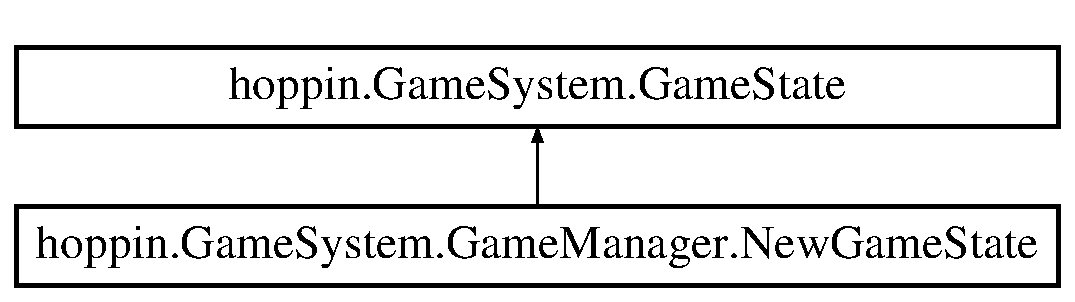
\includegraphics[height=2.000000cm]{classhoppin_1_1_game_system_1_1_game_state}
\end{center}
\end{figure}
\subsection*{Public Member Functions}
\begin{DoxyCompactItemize}
\item 
List$<$ int $>$ {\bfseries Get\+Player\+Score} ()\hypertarget{classhoppin_1_1_game_system_1_1_game_state_a7fd6f968ac6db4620762f1f5071a435b}{}\label{classhoppin_1_1_game_system_1_1_game_state_a7fd6f968ac6db4620762f1f5071a435b}

\end{DoxyCompactItemize}
\subsection*{Public Attributes}
\begin{DoxyCompactItemize}
\item 
Dictionary$<$ Field\+Object, \hyperlink{classhoppin_1_1_game_system_1_1_player_data}{Player\+Data} $>$ {\bfseries player\+Data\+List} = new Dictionary$<$Field\+Object, \hyperlink{classhoppin_1_1_game_system_1_1_player_data}{Player\+Data}$>$()\hypertarget{classhoppin_1_1_game_system_1_1_game_state_a770b9eac31b09a8b05306cbfa31480c7}{}\label{classhoppin_1_1_game_system_1_1_game_state_a770b9eac31b09a8b05306cbfa31480c7}

\item 
List$<$ string $>$ {\bfseries player\+Name} = new List$<$string$>$()\hypertarget{classhoppin_1_1_game_system_1_1_game_state_a3b397e26c99ffb7dc8983277c1020c53}{}\label{classhoppin_1_1_game_system_1_1_game_state_a3b397e26c99ffb7dc8983277c1020c53}

\item 
int {\bfseries Play\+Count} = new int()\hypertarget{classhoppin_1_1_game_system_1_1_game_state_a73a4b19854ff38c7961c21df924de563}{}\label{classhoppin_1_1_game_system_1_1_game_state_a73a4b19854ff38c7961c21df924de563}

\item 
List$<$ \hyperlink{classhoppin_1_1_game_system_1_1_position}{Position} $>$ {\bfseries box\+Position\+List} = new List$<$\hyperlink{classhoppin_1_1_game_system_1_1_position}{Position}$>$()\hypertarget{classhoppin_1_1_game_system_1_1_game_state_aeede9b8f24c849cc4a979ba5e3f1dbb6}{}\label{classhoppin_1_1_game_system_1_1_game_state_aeede9b8f24c849cc4a979ba5e3f1dbb6}

\item 
List$<$ \hyperlink{classhoppin_1_1_game_system_1_1_position}{Position} $>$ {\bfseries shoes\+Position\+List} = new List$<$\hyperlink{classhoppin_1_1_game_system_1_1_position}{Position}$>$()\hypertarget{classhoppin_1_1_game_system_1_1_game_state_aafbf8d917ae66259ead1c2519a757cff}{}\label{classhoppin_1_1_game_system_1_1_game_state_aafbf8d917ae66259ead1c2519a757cff}

\item 
List$<$ \hyperlink{classhoppin_1_1_game_system_1_1_position}{Position} $>$ {\bfseries bonus\+Position\+List} = new List$<$\hyperlink{classhoppin_1_1_game_system_1_1_position}{Position}$>$()\hypertarget{classhoppin_1_1_game_system_1_1_game_state_ade3862019acf3fa56dc394455b087226}{}\label{classhoppin_1_1_game_system_1_1_game_state_ade3862019acf3fa56dc394455b087226}

\end{DoxyCompactItemize}
\subsection*{Protected Attributes}
\begin{DoxyCompactItemize}
\item 
int {\bfseries max\+Turn}\hypertarget{classhoppin_1_1_game_system_1_1_game_state_ac0d86483ff1a4c0d1e3e7433ef6b7a47}{}\label{classhoppin_1_1_game_system_1_1_game_state_ac0d86483ff1a4c0d1e3e7433ef6b7a47}

\item 
Field\+Object\mbox{[},\mbox{]} {\bfseries field\+State} = new Field\+Object\mbox{[}F\+I\+E\+L\+D\+H\+E\+I\+G\+HT,F\+I\+E\+L\+D\+W\+I\+D\+TH\mbox{]}\hypertarget{classhoppin_1_1_game_system_1_1_game_state_a6001d9ae6220bae0ba0831799e3bf96d}{}\label{classhoppin_1_1_game_system_1_1_game_state_a6001d9ae6220bae0ba0831799e3bf96d}

\item 
Field\+Object\mbox{[},\mbox{]} {\bfseries field\+Floor\+Color} = new Field\+Object\mbox{[}F\+I\+E\+L\+D\+H\+E\+I\+G\+HT, F\+I\+E\+L\+D\+W\+I\+D\+TH\mbox{]}\hypertarget{classhoppin_1_1_game_system_1_1_game_state_a6b236f43815ef3fd89072d3b0ea11d33}{}\label{classhoppin_1_1_game_system_1_1_game_state_a6b236f43815ef3fd89072d3b0ea11d33}

\item 
Player\+Move {\bfseries current\+Player\+Move}\hypertarget{classhoppin_1_1_game_system_1_1_game_state_a34e4c930c267e3c1e8be2b33b1fb695b}{}\label{classhoppin_1_1_game_system_1_1_game_state_a34e4c930c267e3c1e8be2b33b1fb695b}

\item 
Field\+Object {\bfseries current\+Player}\hypertarget{classhoppin_1_1_game_system_1_1_game_state_a5057df7ffdb264f8835f209e1b882fc4}{}\label{classhoppin_1_1_game_system_1_1_game_state_a5057df7ffdb264f8835f209e1b882fc4}

\end{DoxyCompactItemize}
\subsection*{Properties}
\begin{DoxyCompactItemize}
\item 
Player\+Move {\bfseries Current\+Player\+Move}\hspace{0.3cm}{\ttfamily  \mbox{[}get\mbox{]}}\hypertarget{classhoppin_1_1_game_system_1_1_game_state_ada3834c6d2c1ccdc3bde5576a441a230}{}\label{classhoppin_1_1_game_system_1_1_game_state_ada3834c6d2c1ccdc3bde5576a441a230}

\item 
Field\+Object {\bfseries Current\+Player}\hspace{0.3cm}{\ttfamily  \mbox{[}get\mbox{]}}\hypertarget{classhoppin_1_1_game_system_1_1_game_state_a556b34d4e6bbaeaadee64a2b37297039}{}\label{classhoppin_1_1_game_system_1_1_game_state_a556b34d4e6bbaeaadee64a2b37297039}

\item 
\hyperlink{classhoppin_1_1_game_system_1_1_player_data}{Player\+Data} {\bfseries Current\+Player\+Data}\hspace{0.3cm}{\ttfamily  \mbox{[}get\mbox{]}}\hypertarget{classhoppin_1_1_game_system_1_1_game_state_aa5d13798c4d9c6cc77089a8b35bcfef7}{}\label{classhoppin_1_1_game_system_1_1_game_state_aa5d13798c4d9c6cc77089a8b35bcfef7}

\item 
int {\bfseries Turn\+Num}\hspace{0.3cm}{\ttfamily  \mbox{[}get, set\mbox{]}}\hypertarget{classhoppin_1_1_game_system_1_1_game_state_a7d5c63680a553530b2b5ede5045a49a0}{}\label{classhoppin_1_1_game_system_1_1_game_state_a7d5c63680a553530b2b5ede5045a49a0}

\item 
int {\bfseries Field\+Width}\hspace{0.3cm}{\ttfamily  \mbox{[}get\mbox{]}}\hypertarget{classhoppin_1_1_game_system_1_1_game_state_af1d1a8a6d4cb794cf0b4314f12720d96}{}\label{classhoppin_1_1_game_system_1_1_game_state_af1d1a8a6d4cb794cf0b4314f12720d96}

\item 
int {\bfseries Field\+Height}\hspace{0.3cm}{\ttfamily  \mbox{[}get\mbox{]}}\hypertarget{classhoppin_1_1_game_system_1_1_game_state_aa6acc094597adc0350a25824b7a9d105}{}\label{classhoppin_1_1_game_system_1_1_game_state_aa6acc094597adc0350a25824b7a9d105}

\item 
int {\bfseries Shoes\+Turn}\hspace{0.3cm}{\ttfamily  \mbox{[}get\mbox{]}}\hypertarget{classhoppin_1_1_game_system_1_1_game_state_af347f2c33f7960789f5c845ed8e6f13c}{}\label{classhoppin_1_1_game_system_1_1_game_state_af347f2c33f7960789f5c845ed8e6f13c}

\item 
Field\+Object\mbox{[},\mbox{]} {\bfseries Field\+State}\hspace{0.3cm}{\ttfamily  \mbox{[}get, set\mbox{]}}\hypertarget{classhoppin_1_1_game_system_1_1_game_state_a2a28e86ec245b55fb6120055e5299cd7}{}\label{classhoppin_1_1_game_system_1_1_game_state_a2a28e86ec245b55fb6120055e5299cd7}

\item 
Field\+Object\mbox{[},\mbox{]} {\bfseries Field\+Floor\+Color}\hspace{0.3cm}{\ttfamily  \mbox{[}get, set\mbox{]}}\hypertarget{classhoppin_1_1_game_system_1_1_game_state_aeb3113972aa024e7929806a6015bf8f7}{}\label{classhoppin_1_1_game_system_1_1_game_state_aeb3113972aa024e7929806a6015bf8f7}

\item 
int {\bfseries Think\+Time}\hspace{0.3cm}{\ttfamily  \mbox{[}get\mbox{]}}\hypertarget{classhoppin_1_1_game_system_1_1_game_state_a13573b010e37d7bb31c8fef8f46b7171}{}\label{classhoppin_1_1_game_system_1_1_game_state_a13573b010e37d7bb31c8fef8f46b7171}

\item 
int {\bfseries Max\+Turn}\hspace{0.3cm}{\ttfamily  \mbox{[}get\mbox{]}}\hypertarget{classhoppin_1_1_game_system_1_1_game_state_ae85e1930a8705706c34e831ea832f6d0}{}\label{classhoppin_1_1_game_system_1_1_game_state_ae85e1930a8705706c34e831ea832f6d0}

\end{DoxyCompactItemize}


\subsection{Detailed Description}
summary$>$ 全ゲーム情報を保持する Game\+Managerが統括する /summary$>$ 

The documentation for this class was generated from the following file\+:\begin{DoxyCompactItemize}
\item 
Game\+System/Game\+State.\+cs\end{DoxyCompactItemize}

\hypertarget{classhoppin_1_1_hoppin_u_i}{}\section{hoppin.\+Hoppin\+UI Class Reference}
\label{classhoppin_1_1_hoppin_u_i}\index{hoppin.\+Hoppin\+UI@{hoppin.\+Hoppin\+UI}}
Inheritance diagram for hoppin.\+Hoppin\+UI\+:\begin{figure}[H]
\begin{center}
\leavevmode
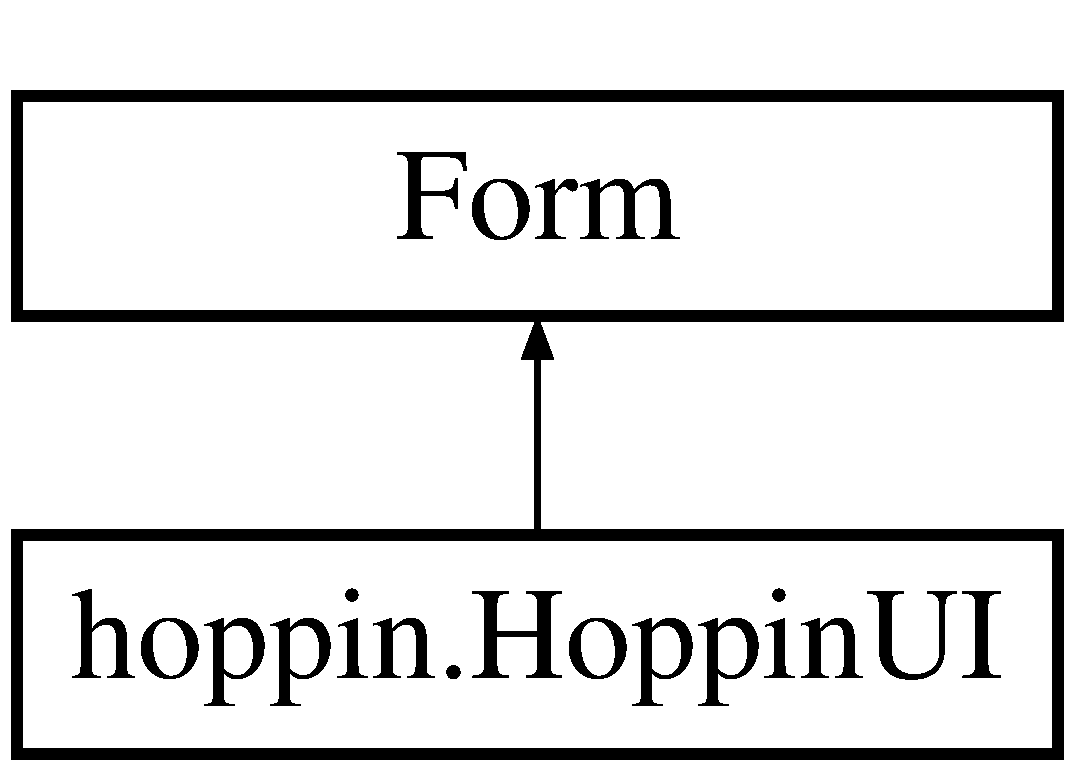
\includegraphics[height=2.000000cm]{classhoppin_1_1_hoppin_u_i}
\end{center}
\end{figure}
\subsection*{Public Member Functions}
\begin{DoxyCompactItemize}
\item 
{\bfseries Hoppin\+UI} (\hyperlink{classhoppin_1_1_game_system_1_1_game_manager}{Game\+Manager} game\+Manager)\hypertarget{classhoppin_1_1_hoppin_u_i_a7faed3d0cc7a679dad7800bd1ab6d4a9}{}\label{classhoppin_1_1_hoppin_u_i_a7faed3d0cc7a679dad7800bd1ab6d4a9}

\end{DoxyCompactItemize}
\subsection*{Protected Member Functions}
\begin{DoxyCompactItemize}
\item 
override void \hyperlink{classhoppin_1_1_hoppin_u_i_a4ebb6fb66a82f87ac8c53665958ba151}{On\+Paint} (Paint\+Event\+Args e)
\begin{DoxyCompactList}\small\item\em 描画インタフェース \end{DoxyCompactList}\item 
override void \hyperlink{classhoppin_1_1_hoppin_u_i_a6bb97d2a8631997b34eb333080958c23}{Dispose} (bool disposing)
\begin{DoxyCompactList}\small\item\em 使用中のリソースをすべてクリーンアップします。 \end{DoxyCompactList}\end{DoxyCompactItemize}


\subsection{Member Function Documentation}
\index{hoppin\+::\+Hoppin\+UI@{hoppin\+::\+Hoppin\+UI}!Dispose@{Dispose}}
\index{Dispose@{Dispose}!hoppin\+::\+Hoppin\+UI@{hoppin\+::\+Hoppin\+UI}}
\subsubsection[{\texorpdfstring{Dispose(bool disposing)}{Dispose(bool disposing)}}]{\setlength{\rightskip}{0pt plus 5cm}override void hoppin.\+Hoppin\+U\+I.\+Dispose (
\begin{DoxyParamCaption}
\item[{bool}]{disposing}
\end{DoxyParamCaption}
)\hspace{0.3cm}{\ttfamily [protected]}}\hypertarget{classhoppin_1_1_hoppin_u_i_a6bb97d2a8631997b34eb333080958c23}{}\label{classhoppin_1_1_hoppin_u_i_a6bb97d2a8631997b34eb333080958c23}


使用中のリソースをすべてクリーンアップします。 


\begin{DoxyParams}{Parameters}
{\em disposing} & マネージ リソースが破棄される場合 true、破棄されない場合は false です。\\
\hline
\end{DoxyParams}
\index{hoppin\+::\+Hoppin\+UI@{hoppin\+::\+Hoppin\+UI}!On\+Paint@{On\+Paint}}
\index{On\+Paint@{On\+Paint}!hoppin\+::\+Hoppin\+UI@{hoppin\+::\+Hoppin\+UI}}
\subsubsection[{\texorpdfstring{On\+Paint(\+Paint\+Event\+Args e)}{OnPaint(PaintEventArgs e)}}]{\setlength{\rightskip}{0pt plus 5cm}override void hoppin.\+Hoppin\+U\+I.\+On\+Paint (
\begin{DoxyParamCaption}
\item[{Paint\+Event\+Args}]{e}
\end{DoxyParamCaption}
)\hspace{0.3cm}{\ttfamily [protected]}}\hypertarget{classhoppin_1_1_hoppin_u_i_a4ebb6fb66a82f87ac8c53665958ba151}{}\label{classhoppin_1_1_hoppin_u_i_a4ebb6fb66a82f87ac8c53665958ba151}


描画インタフェース 


\begin{DoxyParams}{Parameters}
{\em e} & \\
\hline
\end{DoxyParams}


The documentation for this class was generated from the following files\+:\begin{DoxyCompactItemize}
\item 
Game\+System/Hoppin\+U\+I.\+cs\item 
Game\+System/Hoppin\+U\+I.\+Designer.\+cs\end{DoxyCompactItemize}

\hypertarget{classhoppin_1_1_game_system_1_1_judgement}{}\section{hoppin.\+Game\+System.\+Judgement Class Reference}
\label{classhoppin_1_1_game_system_1_1_judgement}\index{hoppin.\+Game\+System.\+Judgement@{hoppin.\+Game\+System.\+Judgement}}
\subsection*{Public Member Functions}
\begin{DoxyCompactItemize}
\item 
{\bfseries Judgement} (\hyperlink{classhoppin_1_1_game_system_1_1_game_state}{Game\+State} game\+State, int player\+Score)\hypertarget{classhoppin_1_1_game_system_1_1_judgement_a69f21fd0959cfd8a41e79fced24d0768}{}\label{classhoppin_1_1_game_system_1_1_judgement_a69f21fd0959cfd8a41e79fced24d0768}

\item 
abstract void {\bfseries Judge\+Player\+Move} ()\hypertarget{classhoppin_1_1_game_system_1_1_judgement_ac2aedd52103fdf68766390f2fb4487a3}{}\label{classhoppin_1_1_game_system_1_1_judgement_ac2aedd52103fdf68766390f2fb4487a3}

\end{DoxyCompactItemize}


The documentation for this class was generated from the following file\+:\begin{DoxyCompactItemize}
\item 
hoppin/\+Game\+System/Judgement.\+cs\end{DoxyCompactItemize}

\hypertarget{classhoppin_1_1_sample_player}{}\section{hoppin.\+Sample\+Player Class Reference}
\label{classhoppin_1_1_sample_player}\index{hoppin.\+Sample\+Player@{hoppin.\+Sample\+Player}}
Inheritance diagram for hoppin.\+Sample\+Player\+:\begin{figure}[H]
\begin{center}
\leavevmode
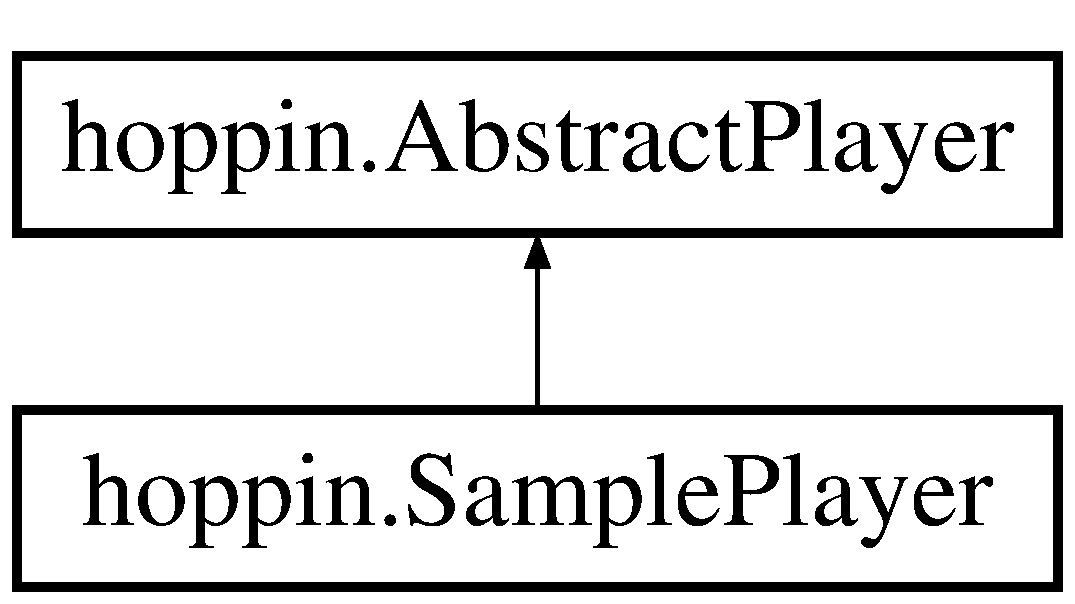
\includegraphics[height=2.000000cm]{classhoppin_1_1_sample_player}
\end{center}
\end{figure}
\subsection*{Public Member Functions}
\begin{DoxyCompactItemize}
\item 
{\bfseries Sample\+Player} (string name)\hypertarget{classhoppin_1_1_sample_player_ab54d749ed27ffe85c01f939cdb4c5c70}{}\label{classhoppin_1_1_sample_player_ab54d749ed27ffe85c01f939cdb4c5c70}

\item 
override Player\+Move {\bfseries move} ()\hypertarget{classhoppin_1_1_sample_player_a6a27c215c5363baf80910f5d44385c7f}{}\label{classhoppin_1_1_sample_player_a6a27c215c5363baf80910f5d44385c7f}

\end{DoxyCompactItemize}
\subsection*{Additional Inherited Members}


The documentation for this class was generated from the following file\+:\begin{DoxyCompactItemize}
\item 
hoppin/\+Sample\+Player/Sample\+Player.\+cs\end{DoxyCompactItemize}

\hypertarget{classhoppin_1_1_game_system_1_1_u_i_1_1_score_board}{}\section{hoppin.\+Game\+System.\+U\+I.\+Score\+Board Class Reference}
\label{classhoppin_1_1_game_system_1_1_u_i_1_1_score_board}\index{hoppin.\+Game\+System.\+U\+I.\+Score\+Board@{hoppin.\+Game\+System.\+U\+I.\+Score\+Board}}
\subsection*{Public Member Functions}
\begin{DoxyCompactItemize}
\item 
{\bfseries Score\+Board} (\hyperlink{classhoppin_1_1_game_system_1_1_game_state}{Game\+State} game\+State)\hypertarget{classhoppin_1_1_game_system_1_1_u_i_1_1_score_board_a8cef263c361863428307f1d378cc5811}{}\label{classhoppin_1_1_game_system_1_1_u_i_1_1_score_board_a8cef263c361863428307f1d378cc5811}

\item 
void {\bfseries draw} (Paint\+Event\+Args e)\hypertarget{classhoppin_1_1_game_system_1_1_u_i_1_1_score_board_a76cab46ef5d0c5b8348b309510d099fa}{}\label{classhoppin_1_1_game_system_1_1_u_i_1_1_score_board_a76cab46ef5d0c5b8348b309510d099fa}

\end{DoxyCompactItemize}


The documentation for this class was generated from the following file\+:\begin{DoxyCompactItemize}
\item 
Game\+System/\+U\+I/Score\+Board.\+cs\end{DoxyCompactItemize}

\hypertarget{classhoppin_1_1_game_system_1_1_u_i_1_1_score_panel}{}\section{hoppin.\+Game\+System.\+U\+I.\+Score\+Panel Class Reference}
\label{classhoppin_1_1_game_system_1_1_u_i_1_1_score_panel}\index{hoppin.\+Game\+System.\+U\+I.\+Score\+Panel@{hoppin.\+Game\+System.\+U\+I.\+Score\+Panel}}
\subsection*{Public Member Functions}
\begin{DoxyCompactItemize}
\item 
{\bfseries Score\+Panel} (String player\+I\+D\+\_\+, Color panel\+Color\+\_\+, String player\+Name\+\_\+, int score\+\_\+, bool active\+\_\+)\hypertarget{classhoppin_1_1_game_system_1_1_u_i_1_1_score_panel_a369891b4ec6f521459b4763814eebe91}{}\label{classhoppin_1_1_game_system_1_1_u_i_1_1_score_panel_a369891b4ec6f521459b4763814eebe91}

\item 
void {\bfseries draw} (Paint\+Event\+Args e)\hypertarget{classhoppin_1_1_game_system_1_1_u_i_1_1_score_panel_a7a983d672c7042c5ea7641b5b737e0ad}{}\label{classhoppin_1_1_game_system_1_1_u_i_1_1_score_panel_a7a983d672c7042c5ea7641b5b737e0ad}

\end{DoxyCompactItemize}


The documentation for this class was generated from the following file\+:\begin{DoxyCompactItemize}
\item 
hoppin/\+Game\+System/\+U\+I/Score\+Panel.\+cs\end{DoxyCompactItemize}

\hypertarget{classhoppin_1_1_game_system_1_1_u_i_1_1_style}{}\section{hoppin.\+Game\+System.\+U\+I.\+Style Class Reference}
\label{classhoppin_1_1_game_system_1_1_u_i_1_1_style}\index{hoppin.\+Game\+System.\+U\+I.\+Style@{hoppin.\+Game\+System.\+U\+I.\+Style}}
\subsection*{Public Attributes}
\begin{DoxyCompactItemize}
\item 
int {\bfseries window\+Width} = 630\hypertarget{classhoppin_1_1_game_system_1_1_u_i_1_1_style_a4360784124b9dbf837322e984e164c03}{}\label{classhoppin_1_1_game_system_1_1_u_i_1_1_style_a4360784124b9dbf837322e984e164c03}

\item 
int {\bfseries window\+Height} = 462\hypertarget{classhoppin_1_1_game_system_1_1_u_i_1_1_style_a80e6ad2d50b7c934a8710a86fdf72886}{}\label{classhoppin_1_1_game_system_1_1_u_i_1_1_style_a80e6ad2d50b7c934a8710a86fdf72886}

\item 
Color {\bfseries background\+Color} = Color.\+White\hypertarget{classhoppin_1_1_game_system_1_1_u_i_1_1_style_ae3e9b970d5840fee32aee2e928e18fe4}{}\label{classhoppin_1_1_game_system_1_1_u_i_1_1_style_ae3e9b970d5840fee32aee2e928e18fe4}

\item 
Color {\bfseries separation\+Color} = Color.\+From\+Argb(255, 179, 179, 179)\hypertarget{classhoppin_1_1_game_system_1_1_u_i_1_1_style_aaaa2c18256cf9dfcb169ed9b87250b24}{}\label{classhoppin_1_1_game_system_1_1_u_i_1_1_style_aaaa2c18256cf9dfcb169ed9b87250b24}

\item 
Color {\bfseries turn\+Board\+Color} = Color.\+From\+Argb(255, 26, 26, 26)\hypertarget{classhoppin_1_1_game_system_1_1_u_i_1_1_style_acb5f5f7ff53860d06a46de6e7dc1cafc}{}\label{classhoppin_1_1_game_system_1_1_u_i_1_1_style_acb5f5f7ff53860d06a46de6e7dc1cafc}

\item 
Color {\bfseries turn\+Board\+Rest\+Color} = Color.\+From\+Argb(255, 51, 51, 51)\hypertarget{classhoppin_1_1_game_system_1_1_u_i_1_1_style_a9d72a42c70ca202f3445cdd3aa6cdc2e}{}\label{classhoppin_1_1_game_system_1_1_u_i_1_1_style_a9d72a42c70ca202f3445cdd3aa6cdc2e}

\item 
Color {\bfseries turn\+Color} = Color.\+From\+Argb(255, 204, 204, 204)\hypertarget{classhoppin_1_1_game_system_1_1_u_i_1_1_style_a7129c567d3fc4ce13d76fe958cd24be7}{}\label{classhoppin_1_1_game_system_1_1_u_i_1_1_style_a7129c567d3fc4ce13d76fe958cd24be7}

\item 
Color {\bfseries score\+Inactive\+Color} = Color.\+From\+Argb(127, 255, 255, 255)\hypertarget{classhoppin_1_1_game_system_1_1_u_i_1_1_style_ae3b2ce83a09717f9cc120beeadb1803b}{}\label{classhoppin_1_1_game_system_1_1_u_i_1_1_style_ae3b2ce83a09717f9cc120beeadb1803b}

\item 
Color {\bfseries score\+Color} = Color.\+White\hypertarget{classhoppin_1_1_game_system_1_1_u_i_1_1_style_ae70c0b59f4b4c46e8b607d3f0bc7355a}{}\label{classhoppin_1_1_game_system_1_1_u_i_1_1_style_ae70c0b59f4b4c46e8b607d3f0bc7355a}

\item 
Color {\bfseries player\+A\+Color} = Color.\+From\+Argb(255, 0, 146, 80)\hypertarget{classhoppin_1_1_game_system_1_1_u_i_1_1_style_a9beeae8f40f2dd52da47f721e1aae5f5}{}\label{classhoppin_1_1_game_system_1_1_u_i_1_1_style_a9beeae8f40f2dd52da47f721e1aae5f5}

\item 
Color {\bfseries player\+B\+Color} = Color.\+From\+Argb(255, 237, 173, 11)\hypertarget{classhoppin_1_1_game_system_1_1_u_i_1_1_style_af9075232db5b4f2474396195833ac1f9}{}\label{classhoppin_1_1_game_system_1_1_u_i_1_1_style_af9075232db5b4f2474396195833ac1f9}

\item 
Color {\bfseries player\+C\+Color} = Color.\+From\+Argb(255, 191, 30, 86)\hypertarget{classhoppin_1_1_game_system_1_1_u_i_1_1_style_aaca65216a76dff0d9a88eb4796cb2bd2}{}\label{classhoppin_1_1_game_system_1_1_u_i_1_1_style_aaca65216a76dff0d9a88eb4796cb2bd2}

\item 
Color {\bfseries player\+D\+Color} = Color.\+From\+Argb(255, 0, 134, 171)\hypertarget{classhoppin_1_1_game_system_1_1_u_i_1_1_style_a6622111d080eb569f679ed415f730c1f}{}\label{classhoppin_1_1_game_system_1_1_u_i_1_1_style_a6622111d080eb569f679ed415f730c1f}

\end{DoxyCompactItemize}


The documentation for this class was generated from the following file\+:\begin{DoxyCompactItemize}
\item 
hoppin/\+Game\+System/\+U\+I/Style.\+cs\end{DoxyCompactItemize}

\hypertarget{classhoppin_1_1_game_system_1_1_u_i_1_1_turn_board}{}\section{hoppin.\+Game\+System.\+U\+I.\+Turn\+Board Class Reference}
\label{classhoppin_1_1_game_system_1_1_u_i_1_1_turn_board}\index{hoppin.\+Game\+System.\+U\+I.\+Turn\+Board@{hoppin.\+Game\+System.\+U\+I.\+Turn\+Board}}
\subsection*{Public Member Functions}
\begin{DoxyCompactItemize}
\item 
void {\bfseries draw} (Paint\+Event\+Args e)\hypertarget{classhoppin_1_1_game_system_1_1_u_i_1_1_turn_board_ad0a4585b0066bffe35ec3c8652a4cfe5}{}\label{classhoppin_1_1_game_system_1_1_u_i_1_1_turn_board_ad0a4585b0066bffe35ec3c8652a4cfe5}

\end{DoxyCompactItemize}


The documentation for this class was generated from the following file\+:\begin{DoxyCompactItemize}
\item 
hoppin/\+Game\+System/\+U\+I/Turn\+Board.\+cs\end{DoxyCompactItemize}

%--- End generated contents ---

% Index
\backmatter
\newpage
\phantomsection
\clearemptydoublepage
\addcontentsline{toc}{chapter}{Index}
\printindex

\end{document}
